\chapter{Elementary counting problems}

\section{Sums and sequences}

Let us call $I_n$ the sum of the first $n$ odd numbers. For example:
$$I_1=1, \quad I_2=1+3=4, \quad I_3=1+3+5=9.$$%
\begin{exercise}\label{Prob:SumImp}
Compute these sums of odd numbers:
  \begin{itemize}  
  \item $I_5=1+3+5+7+9$
  \item $I_{50}=1+3+5+7+\dots+99$
  \item $I_{500}=1+3+5+7+\dots+999$
  \item What is the value of $I_{1000}$ (the sum of the first thousand odd numbers)?
  \item What is the value of $I_n$ (the sum of the first $n$ odd numbers?)
\end{itemize}
\hint{find a pattern}
\end{exercise}
%Sug: Diagramas cuadrangulares. %Fig
\tutpagebreak

\begin{exercise}\label{Prob:SumGau}
Compute the following sums of \emph{consecutive} numbers:
\begin{itemize} 
    \item $1+2+3+4+5+\dots+99+100$.
    \item $1+2+3+4+5+\dots+999+1000$.
    \item $1+2+3+4+5+\dots+(n-2)+(n-1)+n$.    
\end{itemize}
\hint{write the sum again in reverse order to compute twice the required sum}
\end{exercise}

%Sug: Suma dos veces al derecho y en orden inverso:

%Sug: Diagramas triangulares. %Fig:

\begin{exercise}
Compute these sums of numbers in \emph{arithmetic progression}:
\begin{itemize} 
    \item $2+4+6\cdots +2k$.
    \item $7+14+21+\cdots +7k$.
    \item $-16-9-2+5+12+19+26+\cdots +145$.
    \item $\frac{-21}{7} + \frac{-17}{7} + \frac{-13}{7}+ \frac{-9}{7} + \cdots + \frac{11}{7} + \frac{15}{7}$.  
\end{itemize}
\end{exercise}
\tutpagebreak

\begin{exercise}\label{ex:powers-of-two}
What is the value of these sums of numbers in \emph{geometric progression}?:
\begin{itemize}
    \item $1+2+4$
    \item $1+2+4+8+16+32+64$
    \item $1+2+4+8+16+\cdots+1024$
\end{itemize}
\hint{find a pattern, or try using binary numbers}
\end{exercise}

\begin{exercise}
What about these fractions (also in \emph{geometric progression})?:
\begin{itemize}
    \item $\frac{1}{2}+\frac{1}{4}+\frac{1}{8}$
    \item $\frac{1}{2}+\frac{1}{4}+\frac{1}{8}+\frac{1}{16}+\frac{1}{32}$
    \item $\frac{1}{2}+\frac{1}{4}+\frac{1}{8}+\dots +\left(\frac{1}{2}\right)^{15}$    
    \end{itemize}
\hint{can you relate these sums to the ones in the previous exercise?}
\end{exercise}
\tutpagebreak

% \begin{exercise}
% Simplifica las las siguientes sumas de fracciones:
% \begin{itemize} 
%     \item $\frac{1}{2}+\frac{1}{4}+\frac{1}{8}+\dots +\left(\frac{1}{2^{10}}\right)$
%     \item $\frac{2}{3}+\frac{2}{9}+\frac{2}{27}+...+\left(\frac{2}{3^{10}}\right)$
%     \item $\frac{3}{4}+\frac{3}{16}+\frac{3}{64}+...+\left(\frac{3}{4^{10}}\right)$
%     \item $\frac{4}{5}+\frac{4}{25}+\frac{4}{125}+...+\left(\frac{4}{5^{10}}\right)$
%     \end{itemize}
% \end{exercise}

\begin{exercise}
Compute these sums of numbers in \emph{geometric progression}:
\begin{itemize}
    \item $1+2+4+8+16+\dots +2^{10}$.
    \item $1+3+9+27+81+\dots +3^{10}$.
    \item $1+k+k^2+k^3+\dots +k^{10}$.
    \end{itemize}
\hint{write the sums in binary/ternary/$k$-nary numbers and multiply by $k-1$}
\end{exercise}

\begin{exercise}
What is the value of the following sums of fractions in \emph{geometric progression}?:
\begin{itemize} 
    \item $1+\frac{1}{2}+\frac{1}{4}+\frac{1}{8}+\dots +\left(\frac{1}{2}\right)^{10}$.
    \item $1+\frac{1}{3}+\frac{1}{9}+\frac{1}{27}+\dots+\left(\frac{1}{3}\right)^{10}$
    \item $1+\frac{1}{k}+\frac{1}{k^2}+\frac{1}{k^3}+\dots+\left(\frac{1}{k}\right)^{10}$
    \end{itemize}
\end{exercise}
\hint{can you relate these sums to the ones in the previous exercise?}
\tutpagebreak

Consider the sequence of numbers: $$c_n:=\frac{1}{6}n(n+1)(2n+1), \quad n=1,2,3,\dots $$

For example, to obtain $c_5$, we replace $n$ by $5$ in the expression, and we get $$c_5 = \frac{1}{6}5(5+1)(2\cdot5+1) = \frac{1}{6}5(6)(11) = 55.$$ 

\begin{exercise} 
Compute the values of $c_1,c_2,c_3$, and $c_4$.
\end{exercise}

\begin{exercise} 
For some reason $c_n$ is always an integer. This means that the expression $n(n+1)(2n+1)$ is always divisible by $6$. Can you explain why this is the case?
\hint{Separate by prime numbers: show that $n(n+1)(2n+1)$ is divisible by $2$ and by $3$. To show that it is divisible by $3$, 
separate in three cases: $n= 3k$, $n= 3k+1$ and $n= 3k+2$} 
\end{exercise}

\begin{exercise} 
What is the value of the difference between two consecutive terms in the sequence? More concretely, what is the value of $c_k-c_{k-1}$?
\end{exercise}
$$c_k-c_{k-1} = \frac{1}{6}k(k+1)(2k+1)-\frac{1}{6}(k-1)(k)(2k-1) = $$
\tutpagebreak

In the last exercise we obtained that the difference $c_k-c_{k-1} = k^2$ for all $k=2,3,4,\dots$. Equivalently, we obtain that $c_{k}+(k+1)^2=c_{k+1}$ for all $k=1,2,3,4,5\dots$. 

With this result anterior we can obtain a sophisticated formula:

\begin{exercise}
Show that the formula for the sum of the first $n$ squares is given by: $$1^2+2^2+3^2+\cdots+n^2=\frac{1}{6}n(n+1)(2n+1).$$ 
Test it for $n=1,2,3,4$.

Use the previous exercise anterior to conclude that the formula is valid for \emph{all} $n=1,2,3, \dots$.
\end{exercise}
\tutpagebreak

The formula for the sums of cubes is a bit simpler.
\begin{exercise}
\begin{enumerate}
    \item Compute the sum: $$1^3+2^3+3^3+\cdots+10^3.$$
    \item Compute the sum: $$1^3+2^3+3^3+\cdots+100^3.$$ Hint: Test for smaller cases and find a pattern.
    \item Make a conjecture for the formula to compute $c_n = 1^3+2^3+3^3+\cdots+n^3$. 
    \item What is the difference $c_k-c_{k-1}$ between two consecutive elements from your formula?
    \item Conclude that you formula is valid for all $n\geq 1$.
\end{enumerate}
\end{exercise}
\tutpagebreak

\begin{exercise}
Encuentra una fórmula para calcular la suma $$1\cdot2+2\cdot3+3\cdot4+\cdots+n\cdot(n+1).$$
\hint{Can you decompose this sum into two sums that we have already solved?}
\end{exercise}
\tutpagebreak

\begin{exercise}
  Consider $n$ points in the circle and draw the $n(n-1)/2$ chords defined by each pair of points. 
  Suppose that the points are arranged in such a way that no three chords intersect in a single point, 
  as shown in the figures.

\begin{center}
  \begin{tikzpicture}[line cap=round,line join=round,>=triangle 45,x=1.5cm,y=1.5cm]
    \clip(-1.1,-1.1) rectangle (1.1,1.1);
    \draw [line width=1.pt] (0.,0.) circle (1.5cm);
    \draw [line width=1.pt] (-0.6842733454009037,0.7292256089673864)-- (0.6995716435123726,-0.7145624644447803);
    \draw [line width=1.pt] (-0.3147519836675201,-0.9491739507473649)-- (0.09504515717703704,0.9954729620121243);
    \draw [line width=1.pt] (1.,0.)-- (-0.9052766399383212,-0.4248225572894913);
    \draw [fill=black] (1.,0.) circle (1.5pt);
    \draw [fill=black] (0.09504515717703704,0.9954729620121243) circle (1.5pt);
    \draw [fill=black] (-0.6842733454009037,0.7292256089673864) circle (1.5pt);
    \draw [fill=black] (-0.9052766399383212,-0.4248225572894913) circle (1.5pt);
    \draw [fill=black] (-0.3147519836675201,-0.9491739507473649) circle (1.5pt);
    \draw [fill=black] (0.6995716435123726,-0.7145624644447803) circle (1.5pt);
    \end{tikzpicture}
    \hspace{1cm}
    \begin{tikzpicture}[line cap=round,line join=round,>=triangle 45,x=1.5cm,y=1.5cm]
      \clip(-1.1,-1.1) rectangle (1.1,1.1);
      \draw [line width=1.pt] (0.,0.) circle (1.5cm);
      \draw [line width=1.pt] (-0.6842733454009037,0.7292256089673864)-- (0.6995716435123726,-0.7145624644447803);
      \draw [line width=1.pt] (-0.3147519836675201,-0.9491739507473649)-- (0.7421026427511382,0.67028625796877);
      \draw [line width=1.pt] (1.,0.)-- (-0.9052766399383212,-0.4248225572894913);
      \draw [fill=black] (1.,0.) circle (1.5pt);
      \draw [fill=black] (0.7421026427511382,0.67028625796877) circle (1.5pt);
      \draw [fill=black] (-0.6842733454009037,0.7292256089673864) circle (1.5pt);
      \draw [fill=black] (-0.9052766399383212,-0.4248225572894913) circle (1.5pt);
      \draw [fill=black] (-0.3147519836675201,-0.9491739507473649) circle (1.5pt);
      \draw [fill=black] (0.6995716435123726,-0.7145624644447803) circle (1.5pt);
      \end{tikzpicture}

  Valid configuration (left) vs invalid configuration (right).    

\end{center} 

In how many regions is the disk split by the chords? 
  
Compute the cases for $n=1,2,3,4,5$ and formulate a conjecture.
\end{exercise}
  
\begin{exercise}
  Now compute the case $n=6$.
\end{exercise}
\tutpagebreak
  
\begin{exercise}
  Consider the sequence of numbers $$r_n = {n \choose 0} + {n \choose 2} + {n \choose 4}$$
  Recall that the \emph{binomial coefficient} is defined as:
  \begin{itemize}
    \item   ${n \choose k} = \frac{n!}{k! (n-k)!}$,
    where $n!=n(n-1)(n-2) \cdots (2)(1)$ is \emph{$n$ factorial} if $k\leq n$,
    \item ${n \choose k} =0$, if $k>n$.
  \end{itemize}

  Do you wish to change your conjecture?
\end{exercise}
\tutpagebreak

\begin{exercise}
Compute the sum $$\frac{1}{1 \cdot 2}+\frac{1}{2 \cdot 3}+\frac{1}{3 \cdot 4}+\cdots+\frac{1}{999 \cdot 1000}.$$
\hint{Simplify your result and find a pattern.}
\end{exercise}

\begin{exercise}
Calcula la suma $$\frac{1}{1 \cdot 3}+\frac{1}{3 \cdot 5}+\frac{1}{5 \cdot 7}+\cdots+\frac{1}{999 \cdot 1001}.$$
\hint{Simplify your result and find a pattern. Factorize.}
\end{exercise}
\vspace{1.5cm}
\tutpagebreak

The famous \emph{Fibonacci numbers} are defined as follows:
$F_0=0$, $F_1=1$, and for all $n\geq 2$, $$F_n=F_{n-1}+F_{n-2}.$$

\begin{exercise}
Compute the first 11 Fibonacci numbers $(F_0,F_1,F_2,\dots,F_{10})$.
\end{exercise}

\begin{exercise}
Show that $$1+F_0+F_1+F_2+\dots +F_n=F_{n+2}.$$
\hint{Simple induction argument.}
\end{exercise}

\begin{exercise}
Show that for all $n\geq 0$, we have $$F_0^2+F_1^2+F_2^2+\dots +F_n^2=F_{n}F_{n+1}.$$
\hint{Simple induction argument.}
\end{exercise}
\tutpagebreak

\begin{exercise}
Consider now the odd Fibonacci numbers $$(J_1,J_2,J_3,J_4,\dots)=(F_1,F_3,F_5,F_7,\dots)=(1,2,5,13,\dots).$$
Show that $$J_1+J_2+J_3+\cdots + J_{n-2}+J_{n-1}+ 2\cdot J_{n}=J_{n+1}.$$
\hint{Simple induction argument.}
\end{exercise}

\begin{exercise}\begin{enumerate}
    \item Compute the sum: $$4\cdot 1+3\cdot 2+2\cdot 3 + 1\cdot4.$$
    \item Compute the sum: $$6\cdot 1+5\cdot 2+4\cdot 3 + 3\cdot4+ 2 \cdot 5 + 1 \cdot 6.$$
    \item Compute the sum: $$1000\cdot 1+999\cdot 2+998\cdot 3+ \cdots + 998\cdot3+ 999 \cdot 2 + 1000 \cdot 1$$
\end{enumerate}
\hint{Compute initial cases. Draw a Pascal-Tartaglia triangle. Find the computed numbers inside the triangle.}
\end{exercise}

\section{Principios Fundamentales de Conteo}

Los siguientes ejercicios tienen que ver con los {\bf principios fundamentales de conteo}: 
\begin{itemize}
    \item Si debo elegir un elemento de un conjunto $X$ {\bf o} un elemento de un conjunto $Y$, las posibilidades se suman ({\bf principio  aditivo}).
    \item Si debo elegir un elemento de un conjunto $X$ {\bf y} un elemento del conjunto $Y$, esto es lo mismo que elegir una pareja $(x,y)$, $x\in X$ $y\in Y$, por lo que las posibilidades se multiplican ({\bf principio multiplicativo}).
\end{itemize}

\begin{ejercicio}
De la ciudad A hay tres caminos a la ciudad B y cuatro caminos a la ciudad C. De la ciudad C a la D hay dos caminos, y de la ciudad B a la D hay dos caminos. ¿De cuantas formas se puede viajar de A a D?.
\end{ejercicio}
\vspace{4cm}

\begin{ejercicio}
Juan tiene tres sombreros y cuatro gorras de béisbol, siete camisetas, dos shorts, tres pantalones, dos pares de tenis y tres pares de zapatos.

¿De cuántas formas se podría vestir Juan el lunes?
\end{ejercicio}
\vspace{4cm}

\section{Factoriales, coeficientes binomiales y multinomiales}

El siguiente grupito de problemas tiene que ver con los números factoriales. Al número $n!:=n(n-1)(n-2)\cdots (3)(2)(1)$ se le llama $n$ {\bf factorial}. Por ejemplo. $5!=120$ y $6!=720$. Por convención, se establece que un producto sobre un conjunto vacío de factores es $1$, por lo que $0!=1$. Esta convención es de gran ayuda para muchas identidades de conteo.

\begin{ejercicio}
¿De cuántas formas puedo ordenar a seis personas en una fila?
\end{ejercicio}
\vspace{4cm}

%Sug: $6!$.

\begin{ejercicio}
Un equipo de futbol consta de 11 jugadoras. ¿De cuántas formas se puede elegir la lista ordenada de cinco jugadoras que tiraran los penales?
\end{ejercicio}
\vspace{4cm}

Un anagrama de una palabra es otra palabra con las mismas letras pero posiblemente en otro orden. Por ejemplo, de la palabra OSA salen seis anagramas distintos. OSA, OAS, ASO, AOS, SAO y SOA.

\begin{ejercicio}
¿De cuántas formas diferentes se pueden reordenar las letras de las siguientes palabras? 

i). OSO, ii). COSA, iii). COCO, iv). CALACA, v). CALABAZA, vi). MURCIELAGO, vii). SALCHIPAPAS.
\end{ejercicio}

%Sug: Si las letras no se repiten son $n!$. Hay que dividir entre el número de repeticiones.

Todas las respuestas del ejercicio anterior son de la forma $${n\choose k_1, k_2, k_3,\dots, k_r}:= \frac{n!}{k_1!k_2!\dots k_r!},\quad  p_1+p_2+\cdots +p_r = n.$$ A estos números se les llama coeficientes multinomiales. También se les conoce como permutaciones con repetición en algunos textos, y a veces se denotan como  $P _{k_1,k_2,\dots, k_r}$, o bien $P^n_{k_1,k_2,\dots, k_r}$. Sugerimos la notación con los paréntesis

Por ejemplo, para SALCHIPAPAS, $n=11$ porque son once letras en total, $k_1 = 3$ (por que hay  tres A's) $k_2=2, k_3=2,$ (porque hay dos letras P's y dos S') $1=k_4=k_5=k_6=k_7$ (porque L,C,H,I solo aparecen una vez) y obtenemos que el número de anagramas derivados de SALCHIPAPAS es $$\frac{11!}{3!2!2!1!1!1!1!}=\frac{11!}{12} = {11\choose 3, 2, 2, 1, 1, 1, 1}.$$ 


Ahora prestemos atención particular a cuando solo tenemos dos caracteres distintos. 

\begin{ejercicio}
¿Cuántos anagramas hay del fatality de Lui Knag: $(\uparrow,\uparrow,\rightarrow,\uparrow,\uparrow,\rightarrow)$?
\end{ejercicio}
\vspace{1cm}

Una {\bf biyección} es una correspondencia uno-a-uno entre dos conjuntos $X$ y $Y$ con la misma cantidad de elementos. Es decir, a cada elemento del conjunto $X$ le toca uno y solo un elemento del conjunto $Y$.

\begin{ejercicio}
¿Puedes encontrar una biyección entre un conjunto de especial de caminos en el plano y el conjunto de anagramas del fatality de Lui Knag? (Pista: considera una cuadricula de $2 \times 4$)
\end{ejercicio}
\vspace{3cm}

Cuando consideramos únicamente dos tipos de caracteres, con $k_1=k$ repeticiones de uno y $k_2= n-k$ repeticiones del otro, obtenemos los coeficientes binomiales:
$${n\choose k}=\frac{n!}{k!(n-k)!}$$

\section{Contando subconjuntos}

Ahora revisaremos algunos problemas básicos sobre contar conjuntos y subconjuntos. Para esto primero repasemos las definiciones y la notación básica.

\subsection{Definiciones de conjuntos, subconjuntos y ejemplos básicos}

Un {\bf conjunto} $X$ es una colección de elementos. Para describir a un conjunto ponemos a sus elementos dentro de los signos de llave.

Por ejemplo $$X:=\{1,2,3 \}$$ es el conjunto que contiene a los primeros tres números naturales. Los elementos del conjunto $X$ son $1$, $2$ y $3$.

El conjunto $$X:=\{\clubsuit,\vardiamondsuit,\spadesuit,\varheartsuit\}$$ tiene cuatro elementos, los elementos son cada uno de los símbolos de la baraja inglesa.

En un conjunto no importa el orden en que se listan sus elementos. Es decir, $$\{\clubsuit,\vardiamondsuit,\spadesuit,\varheartsuit\} =\{\spadesuit,\clubsuit,\vardiamondsuit,\varheartsuit\}$$ son el mismo conjunto.

Un {\bf subconjunto} $Y$ de otro conjunto $X$  se puede pensar intuitivamente como una subcolección de elementos de $X$. Escribimos $$Y\subseteq X.$$ En un sentido mas concreto, $Y$ es un subconjunto de $X$ si cada elemento de $Y$ está contenido en $X$.

Por ejemplo, tanto el conjunto formado por las figuras negras $Y_1 = \{\clubsuit,\spadesuit\}$ como el conjunto formado por las figuras rojas $Y_2 ={\{\vardiamondsuit,\varheartsuit\} }$ son subconjuntos del conjunto $X=\{\clubsuit,\vardiamondsuit,\spadesuit,\varheartsuit\}$.

En principio se vale considerar conjuntos infinitos. Por ejemplo, el conjunto de números enteros positivos $\mathbb N$ está contenido en el conjunto de números reales $\mathbb R$ y podemos escribir $\mathbb N\subseteq \mathbb R$. Pero no nos espantemos: esto es solo para establecer la notación y por ahora solo estaremos trabajando con conjuntos finitos!

\subsection{El tamaño de un conjunto}

Al numero de elementos de un conjunto $X$ se le llama la cardinalidad de $X$. Si un conjunto $X$ tiene $n$ elementos escribimos $$|X|=n$$

Por ejemplo $$|\{1,2,3\}| = 3,\quad\{0,1,2,3\}| = 4,\quad |\{-1,0,1\}| = 3,\quad |\{\clubsuit\}| = 1$$ 

Hay un conjunto un poco raro pero bastante fundamental que se llama el {\bf conjunto vacío} $\{\}$. Se define como el conjunto que no tiene ningún elemento, es decir $$|\{\}|=0.$$ El conjunto vacío es el único conjunto con cero elementos. Se denota muy frecuentemente con el símbolo $\emptyset$, o bien con las llaves vacías $\{\}$. 

En estas notas vamos a usar las llaves vacías porque nos parece más intuitivo a la vista, que se trata del subconjunto que obtengo cuando no elijo a ningún elemento de cualquier conjunto $X$. 

\subsection{Contando subconjuntos}

Entonces, por ejemplo

\begin{itemize}
    \item El conjunto $\{\clubsuit\}$ solo tiene dos subconjuntos: el  conjunto vacío $\{\}$  y el conjunto $\{\clubsuit\}$. 
    \item El conjunto $[2]:=\{1,2\}$ tiene $4$ subconjuntos: $\{\}$, $\{1\}$, $\{2\}$, y $\{1,2\}$.
    \item El conjunto $[3]:=\{1,2,3\}$ tiene $8$ subconjuntos: $\{\}$, $\{1\}$, $\{2\}$, $\{3\}$, $\{1,2\}$, $\{1,3\}$, $\{2,3\}$, $\{1,2,3\}$.

    \item Como podemos observar de los ejemplos anteriores, todo conjunto $X$ tiene siempre dos subconjuntos "triviales": el conjunto "total" $Y=X$ (cuando se incluyen todos los elementos de $X$) y el conjunto vacío $Y = \{\}$ (cuando no se toma ningún elemento del conjunto).

\end{itemize}


Una forma de entender a todos los subconjuntos de $\{1,2,3\}$ es como ternas de taches y O's, donde ponemos una O si incluímos al elemento en el subconjunto y un tache si no lo incluímos. 

Por ejemplo: podemos representar al subconjunto $\{1,3\}$ como la terna $OXO$, porque se eligió incluir al uno y al tres, pero no al dos. Los subconjuntos $\{3\}$, $\{1,2,3\}$ y el conjunto vacío $\emptyset$, se representan con las ternas $XXO$, $OOO$ y $XXX$, respectivamente.

\begin{ejercicio}
¿Cuántos subconjuntos tiene el conjunto $[4]:=\{1,2,3,4\}$?

¿Cómo representarías al subconjunto $\{2,4\}$ y al subconjunto $\{1,2,3\}$ con $O$'s y $X$'s?
\end{ejercicio}
\vspace{1.5cm}

\begin{ejercicio}
¿Cuántos subconjuntos tiene el conjunto $[6]:=\{1,2,3,4,5,6\}$? (No es necesario listarlos, solo calcular cuántos hay).
\end{ejercicio}
\vspace{1cm}





\begin{ejercicio}
¿Cuántos subconjuntos de tamaño $4$ tiene el conjunto $[6]:=\{1,2,3,4,5,6\}$?

¿Cuántos subconjuntos de tamaño $3$ tiene el conjunto $[6]:=\{1,2,3,4,5,6\}$?

¿Cuántos subconjuntos de tamaño $2$ tiene el conjunto $[6]:=\{1,2,3,4,5,6\}$?

¿Cuántos subconjuntos de tamaño $0$ tiene el conjunto $[6]:=\{1,2,3,4,5,6\}$?
\end{ejercicio}
\vspace{2cm}
%Sug: anagramas OOXXOO con cierta cantidad de O's.

\begin{ejercicio} Demuestra la identidad.
$${n \choose 0}+{n \choose 1}+{n \choose 2}+\cdots + {n \choose n}=2^n.$$
\end{ejercicio}
\vspace{2cm}


\begin{ejercicio}
Un equipo completo de baloncesto consta de nueve jugadoras en total. 

a) ¿De cuántas maneras se puede elegir al conjunto de cinco jugadoras titulares que 
jugarán el siguiente partido?

b) ¿De cuántas maneras se puede elegir una alineación con una capitana y 4 jugadoras titulares?
\end{ejercicio}
\vspace{2cm}

%Sug: a) anagramas de titulares y suplentes TTTTTSSSS. b) anagramas de CTTTTSSSS

% Obs: Se puede contar de dos maneras. Primero elegir la capitana y luego a las titulares, o primero a las titulares y de entre ellas a la capitana.

\section{Separadores}

\begin{ejercicio}
¿De cuántas formas se puede elegir una quíntupla ordenada $(n_1, n_2, n_3, n_4, n_5)$ de cinco enteros no-negativos que sumen $16$?
\end{ejercicio}

\begin{ejercicio}
¿De cuántas formas se puede elegir una quíntupla ordenada $(n_1, n_2, n_3, n_4, n_5)$ de cinco números naturales que sumen $16$?
\end{ejercicio}

Nota: Si en lugar de preguntar por quíntuplas ordenadas  por quíntuplas no-ordenadas , no existe una fórmula cerrada.

% hipervínculo.

\begin{ejercicio}
Si tengo veinte canicas idénticas y voy a repartirlas todas entre mis cinco sobrinos. ¿De cuántas maneras distintas puedo repartir \emph{todas} las canicas?.

¿De cuántas maneras puedo hacerlo, si no puedo dejar a ninguno con cero canicas?

¿De cuántas formas puedo repartir las canicas, si se permite que me quede con algunas canicas?

¿De cuántas formas puedo repartir las canicas, si al sobrino más grande le tengo que dar al menos tres?
\end{ejercicio}
\vspace{4cm}

\section{Permutaciones en círculos}

\begin{ejercicio}
¿De cuantas formas distintas se pueden sentar ocho personas en una mesa redonda?
\end{ejercicio}
\vspace{4cm}

\begin{ejercicio}
¿De cuántas formas se pueden pintar las seis caras de un cubo de seis colores distintos, usando todos los seis colores?

¿Y si tuviéramos ocho colores?
\end{ejercicio}


\section{Contando caminos: Coeficientes binomiales}

Según las reglas para multiplicar polinomios, el binomio $(x+y)$ elevado a la $n=1,2,3$ nos da:

$$(x+y)^0=1,\quad (x+y)^1=x+y,\quad (x+y)^2=x^2+2xy+y^2, \quad (x+y)^3=x^3+3x^2y+3xy^2+y^3.$$

%Obs: Revisar simplificación de términos semejantes.

\begin{ejercicio}
¿Cuál es el coeficiente que acompaña $x^5y^4$ al simplificar $(x+y)^9$?
\end{ejercicio}
%Sug: Comparar xxxyxyxyy con los XXXOXOXOO del problema anterior.
\vspace{2cm}

Los coeficientes de $(x+y)^n$ son los números en el $n$-ésimo renglón del {\bf triángulo de Pascal} (donde el primer renglón corresponde a $n=0$):

$$\begin{array}{ccccccccccccccc}
     &&&&&&& 1 &&&&&&&  \\
    &&&&&& 1 && 1 &&&&&& \\
   &&&&& 1 && 2 && 1 &&&&& \\
  &&&& 1 && 3 && 3 && 1 &&&& \\
 &&& 1 && 4 && 6 && 4 && 1 &&& \\
&& 1 && 5 && 10 && 10 && 5 && 1 &&\\
& 1 && 6 && 15 && 20 && 15 && 6 && 1 &\\
1 && 7 && 21 && 35 && 35 && 21 && 7 && 1\\
&& \vdots && &\vdots && && \vdots && &\vdots
\end{array}$$

Entonces, por ejemplo: $$(x+y)^6=x^6+6x^5y+15x^4y^2+20x^3y^3+15x^2 y^4+6xy^5+y^6.$$

Por esta razón los números que aparecen en el triángulo de Pascal se llaman {\bf coeficientes binomiales}, y se denotan por el símbolo ${n \choose k}$.

$$\begin{array}{ccccccccccccccc}
     &&&&&&& {0 \choose 0} &&&&&&&  \\
    &&&&&& {1 \choose 0} && {1 \choose 1} &&&&&& \\
   &&&&& {2 \choose 0} && {2 \choose 1} && {2 \choose 2} &&&&& \\
  &&&& {3 \choose 0} && {3 \choose 1} && {3 \choose 2} && {3 \choose 3} &&&& \\
 &&& {4 \choose 0} && {4 \choose 1} && {4 \choose 2} && {4 \choose 3} && {4 \choose 4} &&& \\
&& {5 \choose 0} && {5 \choose 1} && {5 \choose 2} && {5 \choose 3} && {5 \choose 4} && {5 \choose 5} &&\\
& {6 \choose 0} && {6 \choose 1} && {6 \choose 2} && {6 \choose 3} && {6 \choose 4} && {6 \choose 5} && {6 \choose 6} &\\
{7 \choose 0} && {7 \choose 1} && {7 \choose 2} && {7 \choose 3} && {7 \choose 4} && {7 \choose 5} && {7 \choose 6} && {7 \choose 7}\\
&& \vdots && &\vdots && && \vdots &&& \vdots
\end{array},$$

La fórmula para el coeficiente binomial es muy sencilla en términos de factoriales:
$${n \choose k}=\frac{n!}{k!(n-k)!}$$

\begin{ejercicio} Demuestra la recursión
$${n \choose k}={n-1 \choose k-1}+{n-1\choose k}$$
\end{ejercicio}

\begin{ejercicio} Considera una cuadrícula de $2\times k$ (como en la Figura).
¿Cuántos caminos distintos hay, que solo avancen una unidad hacia la derecha o una unidad hacia arriba, desde el punto $(0,0)$ al $(k,2)$, para $k=0,1,2,3,\dots$?
\end{ejercicio}

\begin{center}
  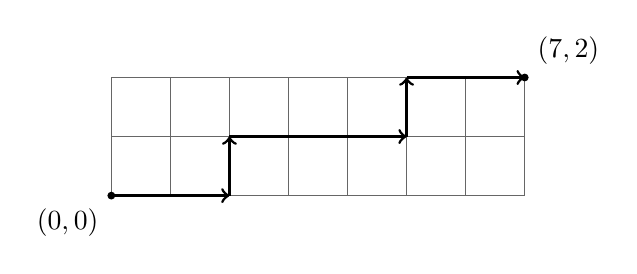
\begin{tikzpicture}[x=0.75cm,y=0.75cm]
    \foreach \i in {0,...,2} \draw[black!60] (0,\i) -- (7,\i);
    \foreach \i in {0,...,7} \draw[black!60] (\i,0) -- (\i,2);

    \draw (0,0) node[circle,fill,inner sep=1pt,label=below left:{$(0,0)$}] {};
    \draw (7,2) node[circle,fill,inner sep=1pt,label=above right:{$(7,2)$}] {};
    \draw[->,line width=1pt] (0,0) -- (2,0);
    \draw[->,line width=1pt] (2,0) -- (2,1);
    \draw[->,line width=1pt] (2,1) -- (5,1);
    \draw[->,line width=1pt] (5,1) -- (5,2);
    \draw[->,line width=1pt] (5,2) -- (7,2);
  \end{tikzpicture}

  $k=7$ y un camino.
\end{center}

%Sug: ¿Cuántos caminos utilizan la subida $(j,0)\uparrow (j,1)$, para cada $j=1,2,3,\dots ,k$?.

\begin{ejercicio} Si se parte del $(0,0)$ y solo se puede mover en cada paso una unidad hacia arriba o hacia la derecha,
\begin{itemize}
    \item ¿Cuántos caminos hay del punto $(0,0)$ al $(2,5)$?.
    \item ¿Cuántos caminos hay del punto $(0,0)$ al $(3,4)$?.
    \item ¿Cuántos caminos hay del punto $(0,0)$ al $(3,5)$?.
\end{itemize}
\end{ejercicio}

\begin{ejercicio}
%ref% [IWYMICI '19]
Mismas reglas: 

¿Cuántos caminos distintos hay del punto $A$ al $B$?

¿Cuántos caminos distintos hay del punto $A$ al $B$, que no pasen por el punto $C$?

\begin{center}
  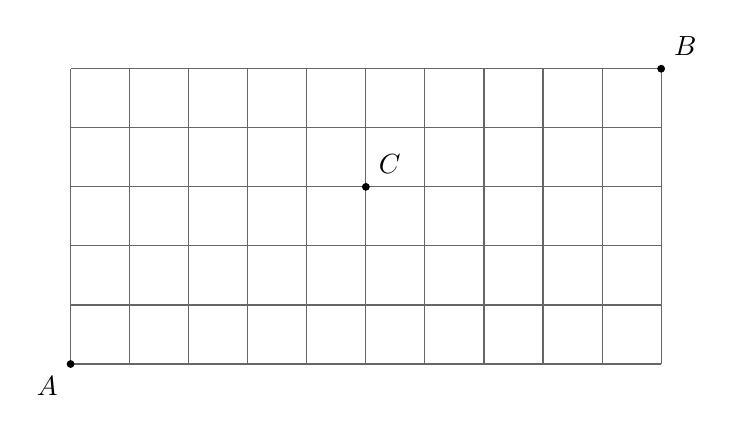
\begin{tikzpicture}[x=0.75cm,y=0.75cm]
    \foreach \i in {0,...,5} \draw[black!60] (0,\i) -- (10,\i);
    \foreach \i in {0,...,10} \draw[black!60] (\i,0) -- (\i,5);

    \draw (0,0) node[circle,fill,inner sep=1pt,label=below left:{$A$}] {};
    \draw (5,3) node[circle,fill,inner sep=1pt,label=above right:{$C$}] {};
    \draw (10,5) node[circle,fill,inner sep=1pt,label=above right:{$B$}] {};
  \end{tikzpicture}
\end{center}
\end{ejercicio}

\begin{ejercicio}
Sea $n$ un número natural. Demostrar siguiente identidad para coeficientes binomiales:
$${2n\choose n}={n \choose 0}^2+{n \choose 1}^2+{n \choose 2}^2+\cdots +{n \choose n}^2.$$
\end{ejercicio}
Sug: ¡Cuenta caminos!
\vspace{4cm}

\begin{ejercicio} Demuestra que para todo $n\geq 1$ se cumple la identidad:
$${n \choose 0}-{n \choose 1}+{n \choose 2}-{n \choose 3}+\cdots +{n \choose n-1}(-1)^{n-1} +{n \choose n}(-1)^n=0.$$
\end{ejercicio}
\vspace{2cm}

\newpage

Varios de los problemas anteriores se pueden resolver directamente usando el teorema del binomio

\begin{teorema}[Teorema del binomio]

Primera versión: $x,y$ números reales o complejos. Entonces se cumple que
$$(x+y)^n={n\choose 0}x^0y^n+{n\choose 1}x^1y^{n-1}+{n\choose 2}x^2y^{n-2}+\dots +{n\choose n}x^ny^0.$$

Versión simplificada ($y=1$): Se tiene que $$(1+x)^n={n\choose 0}x^0+{n\choose 1}x^1+{n\choose 2}x^2+\dots +{n\choose n}x^n.$$
\end{teorema}

\section{Cálculo de probabilidades}

Contar casos favorables entre casos totales es la esencia de la probabilidad discreta. Debido a su aparición frecuente en problemas conteo, los coeficientes binomiales aparecen en muchos problemas elementales de probabilidad.

A veces las probabilidades se presentan en términos de porcentajes. Aunque esto es bastante común, resulta mucho más útil pensar en las probabilidades como números reales entre $0$ y $1$, donde la probabilidad igual a $1$ es equivalente al $100\%$ mientras que la probabilidad igual a $0$ es equivalente al $0\%$.

Por ejemplo, si $X$ es el resultado de lanzar una moneda no truqueada, sabemos que la probabilidad de obtener tanto cara como cruz es de $50\%$ o de $\frac{1}{2}$. De la misma manera, la probabilidad de obtener un $5$ al lanzar un dado es $\frac{1}{6}$.

Es más fácil trabajar con números reales que con porcentajes porque las probabilidades de eventos independientes se multiplican.

Supón que se lanzo una moneda y un dado. ¿Cuál es la probabilidad de obtener una cara y un $2$?

Si lanzo un dado, luego una moneda, luego un dado y luego una moneda, ¿Cuál es la probabilidad de obtener un número par, luego una cara, luego no obtener 3 y luego cruz? 
\vspace{4cm}

\begin{ejercicio} 
En una baraja inglesa de $52$ cartas (con trece cartas de cuatro figuras distintas) calcula la probabilidad de obtener: 
\begin{itemize}
    \item Pokar (cuatro cartas con el mismo número y un número distinto, de una mano de cinco cartas)
    \item Dos pares (distintos y otra carta distinta, en una mano de cinco cartas).
    \item Un full (es decir, una tercia y un par en una mano de cinco cartas).
\end{itemize}.
\end{ejercicio}
\vspace{4cm}

\begin{ejercicio} 
En una baraja inglesa de $52$ cartas (con trece cartas de cuatro figuras distintas) se toman quince cartas.

Se dice que la mano de quince cartas es un churrisflais, si tiene dos tercias, tres pares distintos y tres números distintos.

¿Cuantas conjuntos distintos de quince cartas forman un churrisflais?

¿Cual es la probabilidad de obtener un churrisflais tomando quince cartas al azar?



\end{ejercicio}
\vspace{4cm}

\begin{ejercicio} 
Se lanza una moneda (justa) ocho veces. ¿Cual es la probabilidad de obtener exactamente tres caras?
\end{ejercicio}
\vspace{4cm}

\begin{ejercicio} 
En un casino se encuentran Juan y Sarita, ambos aficionados de la numerología mística. Su número de la suerte es el cuatro. En un arranque, deciden arrojar, cada uno, una moneda justa cuatro veces. Si ambos sacan el mismo número de caras, se casarán de inmediato en la capilla del casino. ¿Con qué probabilidad habrá boda?
\end{ejercicio}
\vspace{4cm}

\begin{ejercicio} 
¿Cuál es la probabilidad de obtener el mismo número de caras si Juan lanza cinco veces una moneda y Sarita la lanza tres veces?
\end{ejercicio}
\vspace{4cm}

\begin{ejercicio} 
Alicia se ubica el punto $(0,0)$ en el plano. Cada minuto lanza un dado y se mueve de acuerdo a la siguiente regla: Si le sale $1$ se mueve a la derecha. Si le sale $2$ o $3$ se mueve hacia la izquierda, y si le sale $4,5$ o $6$ se mueve hacia arriba. ¿Cuál es la probabilidad de que Alicia pise la posición $(1,1)$ por primera vez a los $4$ movimientos? 
\end{ejercicio}
\vspace{4cm}


\begin{ejercicio} 
En la urna A hay una bola blanca y una negra. En la urna B hay tres bolas negras y una blanca. En la urna C hay dos blancas y una negra.

Supón que se elige al azar una bola de la urna A y se mete en la B. Luego se toma a azar una bola de la urna B y se mete en la urna C. Finalmente se extrae una bola al azar de la urna C. ¿Cuál es la probabilidad de que se obtenga una bola negra?
\end{ejercicio}
\vspace{4cm}

\newpage 

\section{Principio de Inclusión y Exclusión}

\begin{ejercicio}
¿Cuántos caminos distintos hay?:
\begin{enumerate}
    \item ¿de $A$ a $B$?
    \item ¿de $A$ a $B$ pasando por $M$ y $N$?
    \item ¿de $A$ a $B$ sin pasar por $M$ ni $N$?
\end{enumerate}
\begin{center}
  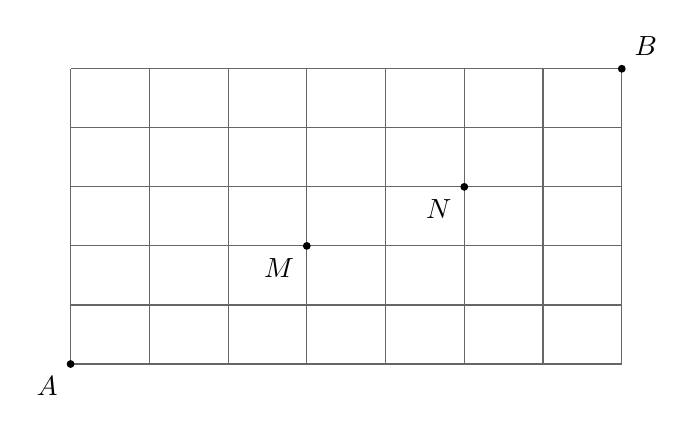
\begin{tikzpicture}[x=1cm,y=0.75cm]
    \foreach \i in {0,...,5} \draw[black!60] (0,\i) -- (7,\i);
    \foreach \i in {0,...,7} \draw[black!60] (\i,0) -- (\i,5);

    \draw (0,0) node[circle,fill,inner sep=1pt,label=below left:{$A$}] {};
    \draw (7,5) node[circle,fill,inner sep=1pt,label=above right:{$B$}] {};
    \draw (3,2) node[circle,fill,inner sep=1pt,label=below left:{$M$}] {};
    \draw (5,3) node[circle,fill,inner sep=1pt,label=below left:{$N$}] {};
  \end{tikzpicture}
\end{center}
\end{ejercicio}
\newpage

\begin{ejercicio}
En un instituto de investigación científica trabajan 67 personas. De estas, 47
hablan inglés, 35 alemán y 23 ambos idiomas. ¿Cuántas personas en el instituto no hablan ni inglés ni alemán?
\end{ejercicio}

\begin{ejercicio}
En un centro de investigación en matemáticas trabajan varias personas, y cada
una de ellas habla por lo menos una lengua extranjera. Seis hablan inglés; seis, alemán; siete, francés. Cuatro hablan inglés y alemán; tres, alemán y francés; dos, francés e inglés. Una persona habla los tres idiomas. 
%Una persona únicamente habla elfo e inglés, pero tiene SNI 3.
¿Cuántas personas trabajan en el centro? ¿Cuántas de ellas hablan solamente inglés?
¿Y solamente francés?
\end{ejercicio}

\begin{tikzpicture}[line cap=round,line join=round,>=triangle 45,x=1.5*1.0cm,y=1.5*1.0cm]
\draw [line width=1.pt] (0.,0.) circle (1.5*1.46cm);
\draw [line width=1.pt] (2.5,0.) circle (1.5*2.28cm);
\draw [line width=1.pt] (0.42,-2.18) circle (1.5*1.9720040567909594cm);
\draw[color=black] (-0.2,0.37) node {$A$};
\draw[color=black] (1.04,0.15) node {$A\cap B$};
\draw[color=black] (2.72,0.51) node {$B$};
\draw[color=black] (.78,-0.53) node {$A\cap B\cap C$};
\draw[color=black] (0.8,-2.01) node {$C$};
\draw[color=black] (1.6,-1.19) node {$B\cap C$};
\draw[color=black] (-0.2,-0.75) node {$A\cap C$};
\end{tikzpicture}

\begin{ejercicio}
Calcula la siguiente suma alternante de coeficientes binomiales:
$${r \choose 1}-{r \choose 2}+{r \choose 3}-{r \choose 4}+\dots \pm {r \choose r}$$
\end{ejercicio}

\begin{teorema}[Principio de inclusión y exclusión]
Sean $A_1,A_2,\dots A_n$ conjuntos, posiblemente con elementos en común.

Entonces 
\begin{equation} \label{Eq:IncExc}
|A_1\cup A_2 \cup \cdots \cup  A_n|=k_1-k_2+k_3-k_4+\dots \pm k_n,
\end{equation}
donde 

$k_1=|A_1|+|A_2|+\dots +|A_n|$,

$k_2=|A_1\cap A_2|+|A_1\cap A_3|+ \dots |A_{n-1}\cap A_n|$

$k_3=|A_1\cap A_2 \cap A_3|+|A_1\cap A_2 \cap A_4|+ \dots |A_{n-2}\cap A_{n-1}\cap A_n|$

$\vdots$

$k_n=|A_1\cap A_2\cap \dots  \cap A_n|$
\end{teorema}

Sugerencia: Primero resuelve el siguiente ejercicio:

\begin{ejercicio}
Supón que un elemento $x\in A_1\cup A_2 \cup \dots \cup A_n$ se encuentra exactamente en $r$ de los conjuntos, digamos $x\in B_1 \cap B_2 \cap B_3 \cdots \cap B_r$, donde los $B_i$'s son algunos de los $A_i$'s.

¿Cuántas veces se cuenta al elemento $x$ en la suma de la ecuación (\ref{Eq:IncExc})?
\end{ejercicio}

\newpage 

\begin{ejercicio}
La función $\varphi(n)$ de Euler cuenta el número enteros positivos $k\leq n$ primos relativos con $n$. Calcula  $\varphi(40)$, $\varphi(120)$, $\varphi(330)$. 
\end{ejercicio}
\vspace{6cm}




%%%%%%%%%%%%%%%%%%%%%%%%%%%%%%%%%%%%%%%%%%%%%%%

\section{Ejercicios}

\begin{ejercicio}
Juan tiene tres sombreros y cuatro gorras de béisbol, siete camisetas, dos shorts, tres pantalones, dos pares de tenis y tres pares de zapatos. Juan es fresa y piensa que <<qué oso>> repetir alguna prenda durante la semana, de lunes a viernes. 

¿De cuantas formas se puede vestir el martes?

¿De cuantas formas puede elegir su outfit de la semana?
\end{ejercicio}

\begin{ejercicio}
¿Cuál es el coeficiente de $x^3y^4z^5$ al expandir el trinomio $(x+y+z)^{12}$?
\end{ejercicio}

\begin{ejercicio}
¿Puedes pensar en un objeto tridimensional análogo al triángulo de Pascal?
\end{ejercicio}

\begin{ejercicio}
Formula el teorema del trinomio: \[(x+y+z)^n=\text{¿qué?}\]
\end{ejercicio}

\begin{ejercicio}
Calcula las potencias $z^n$ del número complejo $z=1+\mathrm i$, para $n=1,2,3,4,5$.
\end{ejercicio}

\begin{ejercicio}
Calcula las potencias $z^n$ del número complejo $z=a+ b\mathrm i$, para $n=1,2,3,4,5$.
\end{ejercicio}

\begin{ejercicio}[Identidad de Vandermonde]
Mostrar que si $m\leq n$ son números naturales, entonces
$${m+n\choose n}={m \choose 0}{n \choose n}+{m \choose 1}{n \choose n-1}+{m \choose 2}{n \choose n-2}+\cdots +{m \choose m-1}{n \choose n-m-1}+{m \choose m}{n \choose n-m}.$$
\end{ejercicio}
%Sug: ¡Cuenta caminos!

\begin{ejercicio}
%[IWYMICT '19]
Hay veinte canicas rojas idénticas, quince canicas negras idénticas y veinte canicas blancas idénticas. Se reparten entre dos niños y una niña. Las condiciones que se deben cumplir son que cada niño reciba al menos dos canicas de cada color y que la niña reciba al menos tres canicas de cada color. 

¿De cuántas maneras se pueden repartir las canicas?
\end{ejercicio}
\newpage

%%%%%%%%%%%%%%%%%%%%%%%%%%%%%%%%%%%%%%%%%%%%%%%
\section{Problemas}

\begin{problema}
%[OMM '87]
¿De cuántas formas se pueden acomodar en una línea recta siete pelotas blancas y cinco negras, de manera que no haya dos pelotas negras juntas?
\end{problema}

\begin{problema}
%[OMM '88]
¿De cuántas formas puedo elegir ocho enteros no necesariamente distintos $a_1, a_2, a_3,\dots ,a_7, a_8$, de tal manera que $1\leq a_1\leq a_2 \leq a_3  \leq  \dots \leq a_7 \leq a_8$?
\end{problema}

\begin{problema}
%[OMM '89]
¿De cuántas formas se puede ir de $A$ a $B$, si solamente se permite ir hacia abajo o hacia los lados, sin pasar dos veces por el mismo punto?

\begin{center}
  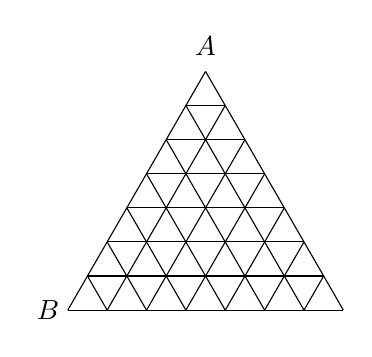
\begin{tikzpicture}[x=.5cm,y=.5cm]
    \foreach \i in {0,...,7} \draw[black] (\i,0) -- (\i*.5,\i*0.866025);
    \foreach \i in {0,...,7} \draw[black] (7-\i,0) -- (7-\i*.5,\i*0.866025);
    \foreach \i in {0,...,7} \draw[black] (0+\i*.5,\i*0.866025) -- (7-\i*.5,\i*0.866025);
    
    \draw[color=black] (-.5,0) node {$B$};
    \draw[color=black] (3.5,6.7) node {$A$};
  \end{tikzpicture}
\end{center}

\end{problema}
\vspace{2cm}

%Sug: Solo importa seleccionar las bajadas, estas determinan las $\to, \leftarrow$ de manera unívoca.

\begin{problema}
%[OMM '00]
Considera un arreglo triangular de números como el siguiente
$$\begin{array}{ccccccccc}
     1 && 2 && 3 && 4 && 5\\
     & 3 && 5 && 7 && 9 &  \\
   && 8 && 12 && 16 &&  \\
  &&& 20 && 28 &&& \\
 &&&& 48 &&&&
\end{array}$$
pero con los números del $1$ al $2000$ en el primer renglón. 

¿Qué número aparece en el vértice inferior del arreglo?
\end{problema}
\vspace{2cm}

%Sug: Dado un número x en en el arreglo,  el número justo dos renglones abajo, en la misma posición, es 4x. 

\begin{problema}
Considera el siguiente tablero de $11 \times 11$: 
\begin{center}
  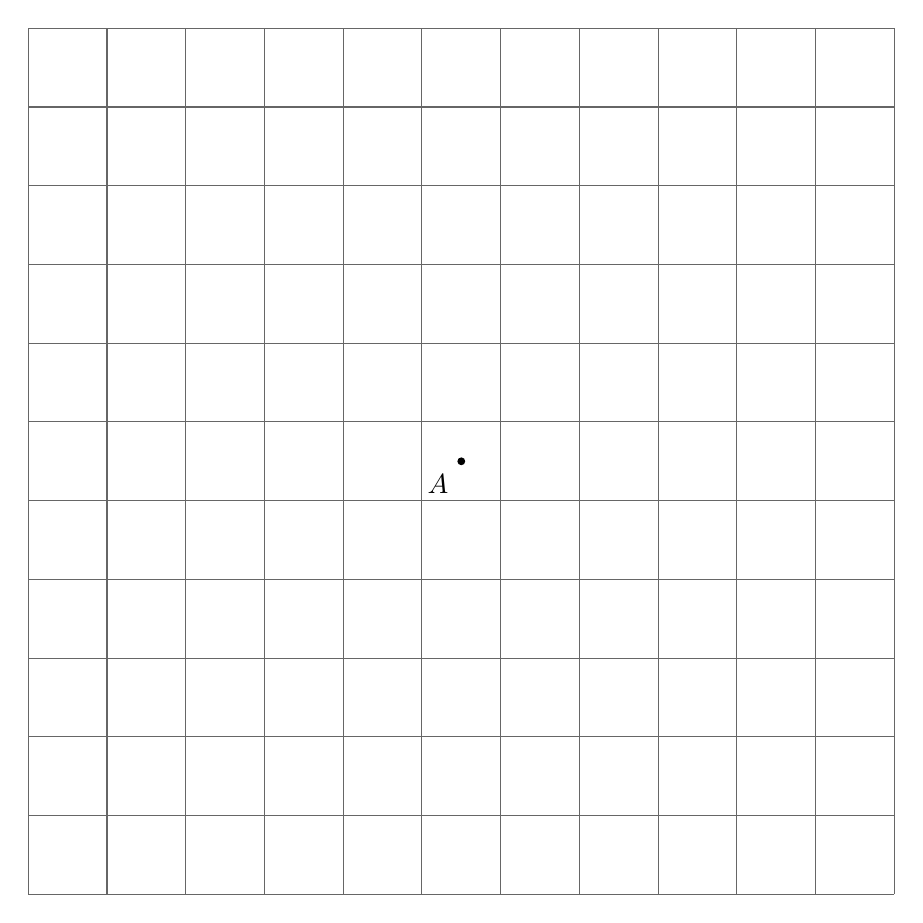
\begin{tikzpicture}[x=1cm,y=1cm]
    \foreach \i in {0,...,11} \draw[black!60] (0,\i) -- (11,\i);
    \foreach \i in {0,...,11} \draw[black!60] (\i,0) -- (\i,11);

    \draw (5.5,5.5) node[circle,fill,inner sep=1pt,label=below left:{$A$}] {};
  \end{tikzpicture}
\end{center}
Alicia se encuentra en la casilla del centro. En cada turno, Alicia arroja un dado en forma de tetraedro con los símbolos $N, S, E, O$ y dependiendo del símbolo que obtenga en el dado se mueve una casilla en esa dirección (Norte, Sur, Este, Oeste).

a) ¿Puede regresar Alicia a la casilla del centro después de exactamente cinco turnos?

b) En cuantas casillas del tablero puede encontrarse Alicia después de exactamente cinco lanzamientos. ¿De cuantas formas distintas puede llegar a cada casilla?

c) Después de cinco lanzamientos Alicia noto que en ninguno de los turnos el paso que dio la dejo mas cercana a la casilla del centro.
¿De cuantas formas distintas pudo moverse Alicia en esos cinco movimientos?
\end{problema}
\vspace{2cm}


\begin{problema}
%[OMM '98]
En el primer paso tomamos un número $n$ y se suman los cuadrados de sus dígitos. En el siguiente paso, se considera el número resultante y se suman los cuadrados de sus dígitos nuevamente, y así sucesivamente. Un número se llama \emph{suertudo} si después de algunos pasos se llega al $1$. 

Por ejemplo, el $1900$ es suertudo pues $$1900 \to 82 \to 68 \to 100 \to 1.$$ 

Encuentra una infinidad de parejas de números consecutivos $(k,k+1)$ donde ambos sean suertudos.
\end{problema}

\begin{problema}
%[OMM '91]
Evalúa la suma de todas las fracciones positivas irreducibles que sean menores que $1$ y que tengan como denominador al $1991$.
\end{problema}

\begin{problema}
%[OMM '93]
La función $f(n,k)$ se define de la siguiente manera:

(1) $f(n,0) = f(n,n) = 1$, y

(2) $f(n,k) = f(n-1,k-1) + f(n-1,k)$ para $0 < k < n$.

¿Cuántas veces se necesita usar la regla (2) para calcular $f(3991,1993)$?
\end{problema}


\begin{problema}
La sucesión $$1, 2, 4, 5, 7, 9 ,10, 12, 14, 16, 17,\dots $$ se forma de la siguiente manera. Primero consideramos un número impar, luego dos pares, luego tres impares, luego cuatro numeros pares, y así sucesivamente. Encuentra el número en la sucesión que se encuentre más cercano a $1994$.
\end{problema}
\vspace{2cm}

\begin{problema}
%[OMM '94]
Los $12$ números en la carátula de un reloj se reacomodan. Muestra que aún se pueden encontrar tres números adyacentes cuya suma es mayor o igual que $21$.
\end{problema}

\begin{problema}
%[OMM '94]
Un matemático bastante payaso, que acababa de leer <<Rayuela>>, escribió un libro con páginas numeradas del $2$ al $400$. Las páginas deben leerse en el siguiente orden. Se toma el número la de última página no leída hasta el momento (al inicio es la $400$) y se leen (en el orden usual) todas las páginas que no son primas relativas a ella, que no se hayan leído antes. El proceso se repite hasta que se leen todas las páginas. Entonces el orden sería $$2, 4, 5,\dots , 400, 3, 7, 9,\dots , 399, \dots$$ ¿Qué página se lee al final?
\end{problema}


\begin{problema}
%[OMM '95]

$N$ estudiantes se sientan en un arreglo de $m \times  n$ donde $m, n \ge  3$. Cada estudiante saluda a cada estudiante vecino horizontalmente, verticalmente y diagonalmente. Si en total hubo $1020$ saludos, ¿cuánto vale $N$?
\end{problema}


\begin{problema}
%[OMM '95]

Encuentra $26$ elementos del conjunto $\{1, 2, 3, ... , 40\}$ de tal forma que el producto de cada dos de ellos nunca sea un cuadrado.
Muestra que no se pueden elegir $27$ elementos con la misma propiedad.
\end{problema}




